\documentclass[a4paper,12pt]{article}
\usepackage[margin=0.5in]{geometry} % This sets the margin to 1 inch on all sides

\usepackage{amsmath}
\usepackage{amssymb}
\usepackage{enumitem}
\usepackage{tikz}
\usetikzlibrary{matrix}

\begin{document}

\title{Arrays e Matrizes}
\author{PCC104 - Projeto e Análise de Algoritmos}
\date{\today}

\maketitle

\section*{Instruções}

\begin{enumerate}
    \item Tente resolver cada um dos exercícios abaixo na complexidade de tempo esperada. Se não conseguir, basta apresentar uma solução qualquer.
    \item Derive a complexidade de tempo e determine a classe de eficiência das soluções propostas.  
\end{enumerate}

\section{Arrays}

\begin{enumerate}

    \item \textbf{Missing in Array} \\
    \textbf{Dificuldade: Fácil} \\
    Dado um array \texttt{arr} de tamanho \( n-1 \) que contém inteiros distintos no intervalo de 1 a \( n \) (inclusive), encontre o elemento faltante. O array é uma permutação de tamanho \( n \) com um elemento faltando. Retorne o elemento faltante.

    \textbf{Exemplos:}
    \begin{itemize}
        \item \textbf{Entrada:} \( n = 5, \texttt{arr} = [1,2,3,5] \) \\
        \textbf{Saída:} 4 \\
        \textbf{Explicação:} Todos os números de 1 a 5 estão presentes, exceto 4.
        
        \item \textbf{Entrada:} \( n = 2, \texttt{arr} = [1] \) \\
        \textbf{Saída:} 2 \\
        \textbf{Explicação:} Todos os números de 1 a 2 estão presentes, exceto 2.
    \end{itemize}
    
    \textbf{Complexidade de Tempo Esperada:} \( O(n) \) \\
    \textbf{Complexidade de Espaço Auxiliar Esperada:} \( O(1) \)

    \item \textbf{Array Leaders} \\
    \textbf{Dificuldade: Fácil} \\
    Dado um array \texttt{arr} de \( n \) inteiros positivos, sua tarefa é encontrar todos os líderes no array. Um elemento do array é considerado um líder se ele for maior que todos os elementos à sua direita ou se for igual ao elemento máximo à sua direita. O elemento mais à direita é sempre um líder.

    \textbf{Exemplos:}
    \begin{itemize}
        \item \textbf{Entrada:} \( n = 6, \texttt{arr} = [16,17,4,3,5,2] \) \\
        \textbf{Saída:} 17 5 2 \\
        \textbf{Explicação:} Não há nada maior à direita de 17, 5 e 2.
        
        \item \textbf{Entrada:} \( n = 5, \texttt{arr} = [10,4,2,4,1] \) \\
        \textbf{Saída:} 10 4 4 1 \\
        \textbf{Explicação:} Ambas as ocorrências de 4 estão na saída, pois ser igual ao maior elemento à direita também é permitido.
    \end{itemize}
    
    \textbf{Complexidade de Tempo Esperada:} \( O(n) \) \\
    \textbf{Complexidade de Espaço Auxiliar Esperada:} \( O(n) \)

    \item \textbf{Second Largest} \\
    \textbf{Dificuldade: Fácil} \\
    Dado um array \texttt{arr}, retorne o segundo maior elemento distinto do array. Se o segundo maior elemento não existir, retorne -1.

    \textbf{Exemplos:}
    \begin{itemize}
        \item \textbf{Entrada:} \texttt{arr} = [12, 35, 1, 10, 34, 1] \\
        \textbf{Saída:} 34 \\
        \textbf{Explicação:} O maior elemento do array é 35 e o segundo maior é 34.
        
        \item \textbf{Entrada:} \texttt{arr} = [10, 10] \\
        \textbf{Saída:} -1 \\
        \textbf{Explicação:} O maior elemento do array é 10 e o segundo maior elemento não existe, então a resposta é -1.
    \end{itemize}
    
    \textbf{Complexidade de Tempo Esperada:} \( O(n) \) \\
    \textbf{Complexidade de Espaço Auxiliar Esperada:} \( O(1) \)

    \item \textbf{Kadane's Algorithm} \\
    \textbf{Dificuldade: Média} \\
    Dado um array de inteiros \texttt{arr[]}. Encontre o subarray contíguo (contendo pelo menos um número) que tem a soma máxima e retorne sua soma.

    \textbf{Exemplos:}
    \begin{itemize}
        \item \textbf{Entrada:} \texttt{arr[]} = [1, 2, 3, -2, 5] \\
        \textbf{Saída:} 9 \\
        \textbf{Explicação:} A soma máxima do subarray é 9, composta pelos elementos [1, 2, 3, -2, 5].
        
        \item \textbf{Entrada:} \texttt{arr[]} = [-1, -2, -3, -4] \\
        \textbf{Saída:} -1 \\
        \textbf{Explicação:} A soma máxima do subarray é -1, composta pelo elemento [-1].
    \end{itemize}
    
    \textbf{Complexidade de Tempo Esperada:} \( O(n) \) \\
    \textbf{Complexidade de Espaço Auxiliar Esperada:} \( O(1) \)

    \item \textbf{Indexes of Subarray Sum} \\
    \textbf{Dificuldade: Média} \\
    Dado um array não ordenado \texttt{arr} de tamanho \( n \) que contém apenas inteiros não-negativos, encontre um subarray (elementos contínuos) que tenha soma igual a \( s \). Você deve retornar os índices esquerdo e direito (indexação baseada em 1) desse subarray.

    No caso de múltiplos subarrays, retorne os índices do subarray que aparece primeiro ao mover da esquerda para a direita. Se nenhum subarray existir, retorne um array contendo o elemento -1.

    \textbf{Exemplos:}
    \begin{itemize}
        \item \textbf{Entrada:} \texttt{arr[]} = [1,2,3,7,5], \( n = 5 \), \( s = 12 \) \\
        \textbf{Saída:} 2 4 \\
        \textbf{Explicação:} A soma dos elementos da 2ª à 4ª posição é 12.
        
        \item \textbf{Entrada:} \texttt{arr[]} = [1,2,3,4,5,6,7,8,9,10], \( n = 10 \), \( s = 15 \)
        \textbf{Saída:} 1 5 \\
        \textbf{Explicação:} A soma dos elementos da 1ª à 5ª posição é 15.
    \end{itemize}
    
    \textbf{Complexidade de Tempo Esperada:} \( O(n) \) \\
    \textbf{Complexidade de Espaço Auxiliar Esperada:} \( O(1) \)

\end{enumerate}

\section{Matrizes}

\begin{enumerate}

    \item \textbf{Search in a Matrix} \\
    \textbf{Dificuldade: Fácil} \\
    Dada uma matriz \texttt{mat[][]} de tamanho \( N \times M \), onde cada linha e coluna está ordenada em ordem crescente, e dado um número \( X \). A tarefa é dizer se o elemento \( X \) está presente na matriz (1) ou não (0).
    
    \textbf{Exemplos:}
    \begin{itemize}
        \item \textbf{Entrada:} \( N = 3, M = 3, \texttt{mat}[][] = \begin{bmatrix}3 & 30 & 38\\44 & 52 & 54\\57 & 60 & 69\end{bmatrix}, X = 62 \) \\
        \textbf{Saída:} 0 \\
        \textbf{Explicação:} 62 não está presente na matriz, então a saída é 0.
        
        \item \textbf{Entrada:} \( N = 1, M = 6, \texttt{mat}[][] = \begin{bmatrix}18 & 21 & 27 & 38 & 55 & 67\end{bmatrix}, X = 55 \) \\
        \textbf{Saída:} 1 \\
        \textbf{Explicação:} 55 está presente na matriz na 5ª célula.
    \end{itemize}
    
    \textbf{Complexidade de Tempo Esperada:} \( O(N+M) \) \\
    \textbf{Complexidade de Espaço Auxiliar Esperada:} \( O(1) \)

    \item \textbf{Transpose of Matrix} \\
    \textbf{Dificuldade: Fácil} \\
    Escreva um programa para encontrar a transposta de uma matriz quadrada de tamanho \( N \times N \). A transposta de uma matriz é obtida trocando-se linhas por colunas e vice-versa.

    \textbf{Exemplos:}
    \begin{itemize}
        \item \textbf{Entrada:} \[ N = 4, \texttt{mat}[][] = 
        \begin{bmatrix}
            1 & 1 & 1 & 1\\
            2 & 2 & 2 & 2\\
            3 & 3 & 3 & 3\\
            4 & 4 & 4 & 4
        \end{bmatrix}\] 

        \textbf{Saída:} 
        \[
        \begin{bmatrix}
            1 & 2 & 3 & 4\\
            1 & 2 & 3 & 4\\
            1 & 2 & 3 & 4\\
            1 & 2 & 3 & 4
        \end{bmatrix}
        \] 
        
        \item \textbf{Entrada:} \( N = 2, \texttt{mat}[][] = \begin{bmatrix}1 & 2\\-9 & -2\end{bmatrix} \) \\
        \textbf{Saída:} 
        \[\begin{bmatrix}
            1 & -9\\
            2 & -2
        \end{bmatrix}\]
    \end{itemize}
    
    \textbf{Complexidade de Tempo Esperada:} \( O(N \times N) \) \\
    \textbf{Complexidade de Espaço Auxiliar Esperada:} \( O(1) \)

    \pagebreak

    \item \textbf{Print Matrix in Snake Pattern} \\
    \textbf{Dificuldade: Fácil} \\
    Dada uma matriz de tamanho \( N \times N \). Imprima os elementos da matriz no padrão serpente (snake pattern) como descrito abaixo.

    \begin{figure}[!ht]
        \centering
    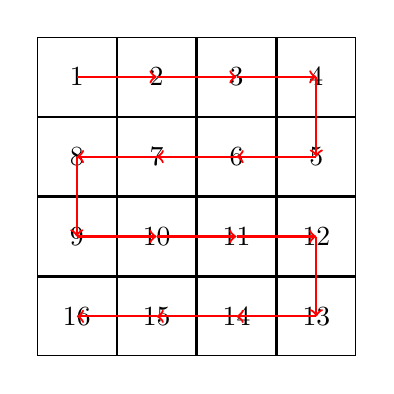
\begin{tikzpicture}
        \matrix (m) [matrix of nodes, nodes in empty cells, nodes={minimum width=1cm, minimum height=1cm, anchor=center, draw}] {
             1 & 2 & 3 & 4 \\
             8 & 7 & 6 & 5 \\
             9 & 10 & 11 & 12 \\
             16 & 15 & 14 & 13 \\
        };
    
        \draw[red, thick, ->] (m-1-1.center) -- (m-1-2.center);
        \draw[red, thick, ->] (m-1-2.center) -- (m-1-3.center);
        \draw[red, thick, ->] (m-1-3.center) -- (m-1-4.center);
        \draw[red, thick, ->] (m-1-4.center) -- (m-2-4.center);
        \draw[red, thick, ->] (m-2-4.center) -- (m-2-3.center);
        \draw[red, thick, ->] (m-2-3.center) -- (m-2-2.center);
        \draw[red, thick, ->] (m-2-2.center) -- (m-2-1.center);
        \draw[red, thick, ->] (m-2-1.center) -- (m-3-1.center);
        \draw[red, thick, ->] (m-3-1.center) -- (m-3-2.center);
        \draw[red, thick, ->] (m-3-2.center) -- (m-3-3.center);
        \draw[red, thick, ->] (m-3-3.center) -- (m-3-4.center);
        \draw[red, thick, ->] (m-3-4.center) -- (m-4-4.center);
        \draw[red, thick, ->] (m-4-4.center) -- (m-4-3.center);
        \draw[red, thick, ->] (m-4-3.center) -- (m-4-2.center);
        \draw[red, thick, ->] (m-4-2.center) -- (m-4-1.center);
    \end{tikzpicture}
    \end{figure}
    

    \textbf{Exemplos:}
    \begin{itemize}
        \item \textbf{Entrada:} \( N = 3, \texttt{mat}[][] = \begin{bmatrix}45 & 48 & 54\\21 & 89 & 87\\70 & 78 & 15\end{bmatrix} \) \\
        \textbf{Saída:} 45 48 54 87 89 21 70 78 15 \\
        \textbf{Explicação:} A matriz é como abaixo: \\
        \[
        \begin{bmatrix}
        45 & 48 & 54 \\
        21 & 89 & 87 \\
        70 & 78 & 15
        \end{bmatrix}
        \]
        Imprimindo no padrão serpente, temos a saída como 45 48 54 87 89 21 70 78 15.
        
        \item \textbf{Entrada:} \( N = 2, \texttt{mat}[][] = \begin{bmatrix}1 & 2\\3 & 4\end{bmatrix} \) \\
        \textbf{Saída:} 1 2 4 3 \\
        \textbf{Explicação:} A matriz é como abaixo: \\
        \[
        \begin{bmatrix}
        1 & 2 \\
        3 & 4
        \end{bmatrix}
        \]
        Imprimindo no padrão serpente, temos a saída como 1 2 4 3.
    \end{itemize}
    
    \textbf{Complexidade de Tempo Esperada:} \( O(N \times N) \) \\
    \textbf{Complexidade de Espaço Auxiliar Esperada:} \( O(N \times N) \) apenas para a lista resultante.

    \item \textbf{Row with Minimum Number of 1's} \\
\textbf{Dificuldade: Fácil} \\
Dada uma matriz binária 2D (indexada a partir de 1) de dimensões \( n \times m \), determine a linha que contém o menor número de 1's. 

\textbf{Nota:} A matriz contém apenas 1's e 0's. Se duas ou mais linhas contiverem o menor número de 1's, a resposta é o menor desses índices.

\textbf{Exemplos:}
\begin{itemize}
    \item \textbf{Entrada:} \( n = 4, m = 4, \texttt{mat}[][] = \begin{bmatrix}1 & 1 & 1 & 1\\1 & 1 & 0 & 0\\0 & 0 & 1 & 1\\1 & 1 & 1 & 1\end{bmatrix} \) \\
    \textbf{Saída:} 2 \\
    \textbf{Explicação:} As linhas 2 e 3 contêm o menor número de 1's (2 cada). Como a linha 2 é menor que a linha 3, a resposta é 2.
    
    \item \textbf{Entrada:} \( n = 3, m = 3, \texttt{mat}[][] = \begin{bmatrix}0 & 0 & 0\\0 & 0 & 0\\0 & 0 & 0\end{bmatrix} \) \\
    \textbf{Saída:} 1 \\
    \textbf{Explicação:} Todas as linhas contêm o mesmo número de 1's (0 cada). Entre elas, o índice 1 é o menor, então a resposta é 1.
\end{itemize}

\textbf{Complexidade de Tempo Esperada:} \( O(n \times m) \) \\
\textbf{Complexidade de Espaço Auxiliar Esperada:} \( O(1) \)

\item \textbf{Rotate by 90 Degree} \\
\textbf{Dificuldade: Média} \\
Dada uma matriz quadrada \texttt{mat[][]} de tamanho \( N \times N \). A tarefa é rotacioná-la em 90 graus no sentido anti-horário sem usar nenhum espaço extra.

\textbf{Exemplos:}
\begin{itemize}
    \item \textbf{Entrada:} \( N = 3, \texttt{mat}[][] = \begin{bmatrix}1 & 2 & 3\\4 & 5 & 6\\7 & 8 & 9\end{bmatrix} \) \\
    \textbf{Saída:} 
    \[
    \begin{bmatrix}
       3 & 6 & 9 \\
       2 & 5 & 8 \\
       1 & 4 & 7 \\
    \end{bmatrix}
    \]
\end{itemize}

\textbf{Complexidade de Tempo Esperada:} \( O(N \times N) \) \\
\textbf{Complexidade de Espaço Auxiliar Esperada:} \( O(1) \)

\item \textbf{Find Whether Path Exists} \\
\textbf{Dificuldade: Média} \\
Dada uma grade de tamanho \( n \times n \) preenchida com 0, 1, 2, 3. Verifique se há um caminho possível do ponto de origem ao destino. Você pode percorrer para cima, para baixo, para a direita e para a esquerda. 

\textbf{Descrição das Células:}
\begin{itemize}
    \item Um valor de célula 1 significa Origem.
    \item Um valor de célula 2 significa Destino.
    \item Um valor de célula 3 significa célula vazia.
    \item Um valor de célula 0 significa Parede (célula bloqueada que não pode ser atravessada).
\end{itemize}

\textbf{Nota:} Há apenas uma única origem e um único destino.

\textbf{Exemplos:}
\begin{itemize}
    \item \textbf{Entrada:} \texttt{grid} = \(\begin{bmatrix}3 & 0 & 3 & 0 & 0\\3 & 0 & 0 & 0 & 3\\3 & 3 & 3 & 3 & 3\\0 & 2 & 3 & 0 & 0\\3 & 0 & 0 & 1 & 3\end{bmatrix}\) \\
    \textbf{Saída:} 0 \\
    \textbf{Explicação:} A grade é como abaixo: \\
    \[
    \begin{bmatrix}
    3 & 0 & 3 & 0 & 0 \\
    3 & 0 & 0 & 0 & 3 \\
    3 & 3 & 3 & 3 & 3 \\
    0 & 2 & 3 & 0 & 0 \\
    3 & 0 & 0 & 1 & 3
    \end{bmatrix}
    \]
    Não há caminho para chegar ao destino (3,1) a partir da origem (4,3).
    
    \item \textbf{Entrada:} \texttt{grid} = \(\begin{bmatrix}1 & 3\\3 & 2\end{bmatrix}\) \\
    \textbf{Saída:} 1 \\
    \textbf{Explicação:} A grade é como abaixo: \\
    \[
    \begin{bmatrix}
    1 & 3 \\
    3 & 2
    \end{bmatrix}
    \]
    Há um caminho da origem (0,0) ao destino (1,1).
\end{itemize}

\textbf{Complexidade de Tempo Esperada:} \( O(n^2) \) \\
\textbf{Complexidade de Espaço Auxiliar Esperada:} \( O(n^2) \)

    
\end{enumerate}

\end{document}
